\documentclass{recipe}

\begin{document}
\begin{recipe}{Fish Sandwich}
  \servings{1}

  \begin{ingredients}
    \ingredient{1}{fillet}{swai}
    \ingredient{\nicefrac{3}{4}}{tbsp}{butter}
    \ingredient{}{}{flour}
    \ingredient{}{}{paprika}
    \ingredient{}{}{garlic powder}
    \ingredient{}{}{onion powder}
    \ingredientsep
    \ingredient{2}{slices}{bread}
    \ingredient{}{}{tarter sauce}
  \end{ingredients}

  \begin{images}
    \begin{image}
      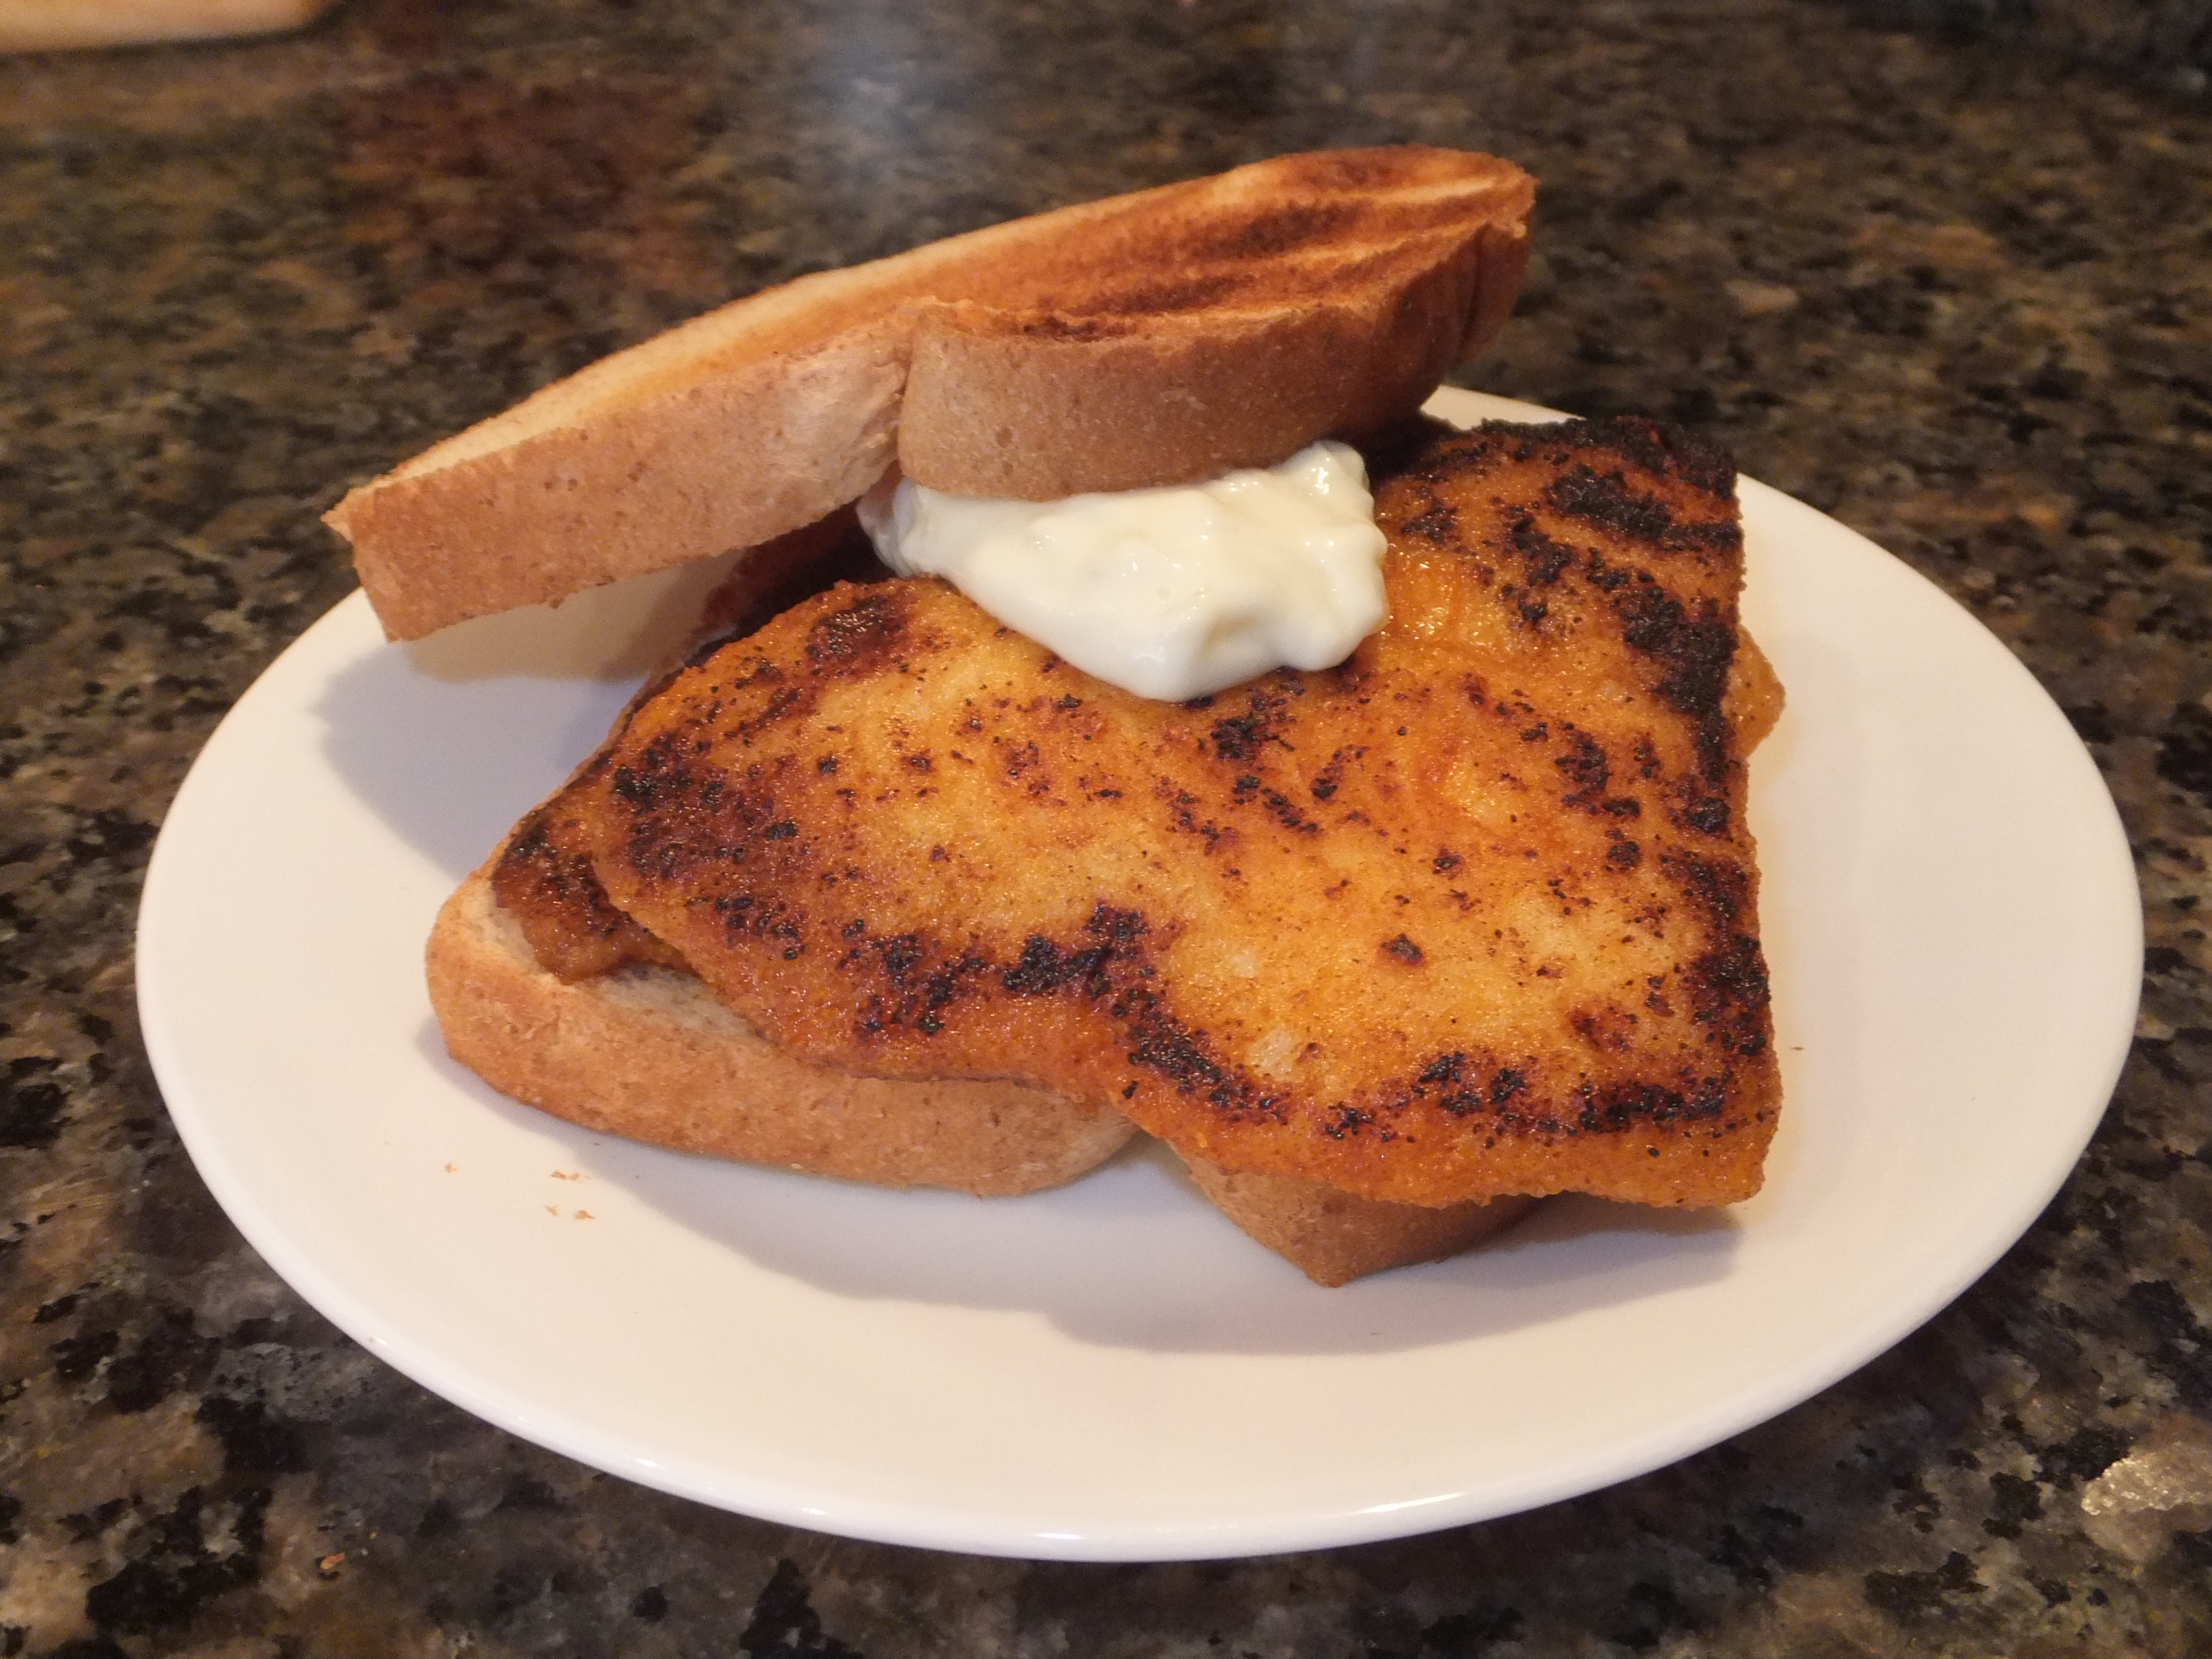
\includegraphics[width=\linewidth,trim=100px 50px 0px 100px, clip=true]{fish_sandwich-01.jpeg}
    \end{image}
  \end{images}

  \begin{steps}
  \item Mix the flour and spices together, dry the fish, and coat it
    in the spice mixture.
  \item Heat a frying pan on high and let it heat up a bit
  \item Melt \nicefrac{1}{2} tablespoon of butter in the pan and let
    it melt but not get brown.
  \item Place the fish in the pan, flat side down
  \item Cook until the fish becomes dark brown on the bottom, but be
    careful because it burns easily.
  \item Add the remaining butter to the pan
  \item Flip the fish over, remove the pan from the heat, and allow
    the fish to cook all the way through with just the heat of the pan
    that remains.
  \item Serve on bread with tarter sauce.
  \end{steps}
\end{recipe}
\end{document}
